\tikzstyle{pvalue}=[circle, draw, fill=blue!50, minimum height=3em]
\tikzstyle{ovalue}=[circle, draw,fill=red!50, minimum height=3em]
\tikzstyle{dcell}=[circle,draw, minimum height=1em]
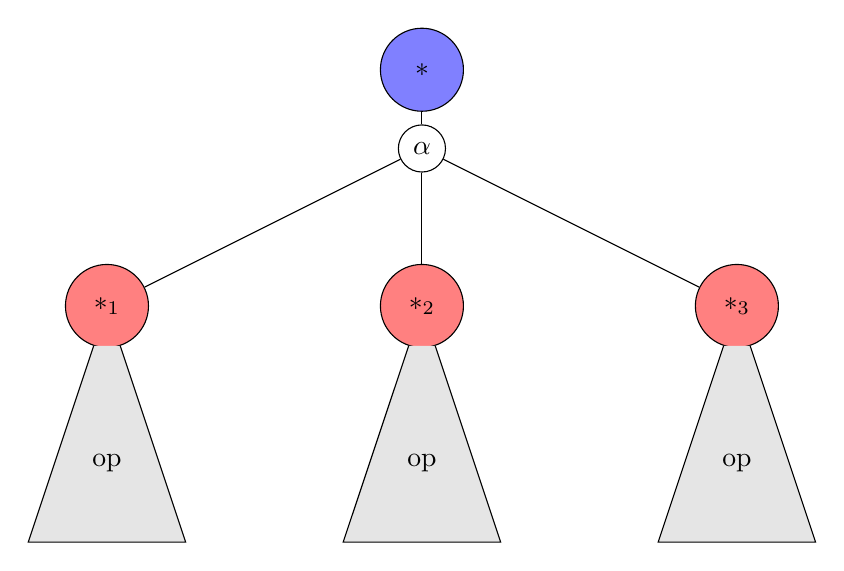
\begin{tikzpicture}

\node[ovalue] (v3) at (8,1) {$\Large{*_3}$};
\draw[draw,fill=gray!20] (v3) -- (7,-2) -- (9,-2) -- (v3) -- cycle;

\node[ovalue] (v2) at (4,1) {$\Large{*_2}$};
\draw[draw,fill=gray!20] (v2) -- (3,-2) -- (5,-2) -- (v2) -- cycle;

\node[ovalue] (v1) at (0,1) {$\Large{*_1}$};
\draw[draw,fill=gray!20] (v1) -- (-1,-2) -- (1,-2) -- (v1) -- cycle;
\node[pvalue] (v4) at (4,4) {$\Large{*}$};
\node[dcell] (v5) at (4,3) {$\alpha$};
\draw  (v4) edge (v5);
\draw  (v5) edge (v1);
\draw  (v2) edge (v5);
\draw  (v3) edge (v5);
\node at (0,-1) {op};
\node at (4,-1) {op};
\node at (8,-1) {op};
\end{tikzpicture}